\documentclass[11pt,a4paper]{article}

\usepackage[margin=2.2cm]{geometry}
\usepackage{amsmath,amssymb,amsthm}
\usepackage{booktabs}
\usepackage{array}
\usepackage{tabularx}
\usepackage[shortlabels]{enumitem}
\usepackage{xcolor}
\usepackage{tikz}
\usepackage{fancyhdr}
\usepackage{setspace}
\usepackage{microtype}
\usepackage{titlesec}
\usepackage{hyperref}
\usepackage{listings}
\usepackage[skins,breakable]{tcolorbox}

\usetikzlibrary{positioning,arrows.meta,calc,fit,shapes.geometric,matrix,decorations.pathreplacing}

\definecolor{ink}{HTML}{222222}
\definecolor{rulegray}{HTML}{444444}
\definecolor{boxline}{HTML}{666666}
\definecolor{boxfill}{HTML}{F4F4F4}
\definecolor{boxtitle}{HTML}{E8E8E8}
\definecolor{g1}{HTML}{D0D0D0}
\definecolor{g2}{HTML}{9A9A9A}
\definecolor{g3}{HTML}{5A5A5A}

\hypersetup{
  colorlinks=true,
  linkcolor=black,
  urlcolor=black,
  pdftitle={MTL 458 Lecture 16: Concurrency},
  pdfauthor={Minati De, IIT Delhi}
}

\setstretch{1.12}
\raggedbottom
\setlist[itemize]{leftmargin=1.3em,itemsep=0.28em,topsep=0.35em}
\setlist[enumerate]{leftmargin=1.5em,itemsep=0.35em,topsep=0.4em}

\titleformat{\section}
  {\Large\bfseries\color{ink}}{\thesection.}{0.6em}{}
  [{\color{rulegray}\titlerule[0.5pt]}]
\titleformat{\subsection}
  {\large\bfseries\color{ink}}{\thesubsection}{0.55em}{}
\titleformat{\subsubsection}
  {\normalsize\bfseries\color{ink}}{\thesubsubsection}{0.5em}{}

\titlespacing*{\section}{0pt}{1.35em}{0.7em}
\titlespacing*{\subsection}{0pt}{1.05em}{0.45em}

\pagestyle{fancy}
\fancyhf{}
\renewcommand{\headrulewidth}{0.4pt}
\renewcommand{\footrulewidth}{0.3pt}
\fancyhead[L]{\small\color{ink}MTL 458 \textbullet\ Operating Systems}
\fancyhead[R]{\small\color{ink}Lecture 16: Concurrency}
\fancyfoot[C]{\small\thepage}
\setlength{\headheight}{14pt}

% ---------------------------------------------------------------------------
% Boxes
% ---------------------------------------------------------------------------
\tcbset{
  commonbox/.style={
    colback=boxfill, colframe=boxline, boxrule=0.5pt,
    left=6pt, right=6pt, top=5pt, bottom=5pt,
    fonttitle=\bfseries, coltitle=black, colbacktitle=boxtitle,
    enhanced, sharp corners=south, breakable
  }
}
\newtcolorbox{keybox}[1][]{commonbox, title={#1}}
\newtcolorbox{quizbox}[1][]{commonbox, title={#1}}
\newtcolorbox{solbox}[1][]{commonbox, title={#1}}
\newtcolorbox{warnbox}[1][]{commonbox, title={#1}}
\newtcolorbox{defbox}[1][]{commonbox, title={#1}}

\lstset{
  language=C,
  basicstyle=\ttfamily\small,
  keywordstyle=\bfseries,
  commentstyle=\itshape\color{g3},
  numbers=left, numberstyle=\scriptsize\color{g2}, numbersep=6pt,
  frame=single, rulecolor=\color{boxline},
  backgroundcolor=\color{boxfill},
  xleftmargin=1.6em, framexleftmargin=1.4em,
  columns=fullflexible, keepspaces=true,
  showstringspaces=false, breaklines=true,
  aboveskip=0.6em, belowskip=0.6em
}
\lstdefinestyle{term}{language={}, numbers=none, basicstyle=\ttfamily\footnotesize,
  xleftmargin=0.4em, framexleftmargin=0.2em}

% Start a new page unless at least #1 of vertical space remains
\makeatletter
\newcommand{\keepspace}[1]{\par\penalty-100\begingroup
  \setlength{\dimen@}{#1}\dimen@ii\pagegoal\advance\dimen@ii-\pagetotal
  \ifdim\dimen@>\dimen@ii\ifdim\dimen@ii>\z@\vfil\fi\break\fi\endgroup}
\makeatother

\newcommand{\eax}{\texttt{\%eax}}
\newcommand{\rip}{\texttt{\%rip}}

\begin{document}

% ===========================================================================
% Title
% ===========================================================================
\begin{center}
{\color{rulegray}\rule{\textwidth}{1.1pt}}\\[0.45em]
{\LARGE\bfseries Operating Systems}\\[0.25em]
{\Large\bfseries MTL 458 \textperiodcentered\ Lecture 16}\\[0.35em]
{\LARGE\bfseries Concurrency}\\[0.35em]
{\large Minati De}\\[0.15em]
{\normalsize Department of Mathematics, Indian Institute of Technology Delhi}\\[0.35em]
{\color{rulegray}\rule{\textwidth}{1.1pt}}
\end{center}

\vspace{0.4em}
\begin{keybox}[What this lecture solves]
We finish the first ``easy piece'' (virtualization) and start the second:
\textbf{concurrency}. The questions:
\begin{itemize}
  \item Why do we need concurrency at all? (CPU trends: more cores, not
        faster cores.)
  \item How do we write one application that uses many CPUs?
        \textbf{Processes} vs.\ a new abstraction, the \textbf{thread}.
  \item What do threads of the same process \textbf{share}, and what is
        \textbf{private}?
  \item The POSIX thread API: \texttt{pthread\_create},
        \texttt{pthread\_join}, \texttt{pthread\_exit}.
  \item Why a shared counter gives the \textbf{wrong answer}: race
        conditions, non-determinism, critical sections, and the need for
        \textbf{atomicity} / \textbf{mutual exclusion}.
\end{itemize}
\end{keybox}

\tableofcontents
\vspace{0.6em}
\noindent{\color{rulegray}\rule{\textwidth}{0.4pt}}

% ===========================================================================
\section{Review: easy piece 1 --- virtualization}
% ===========================================================================

Everything so far in the course has been about \textbf{virtualization}:

\begin{center}
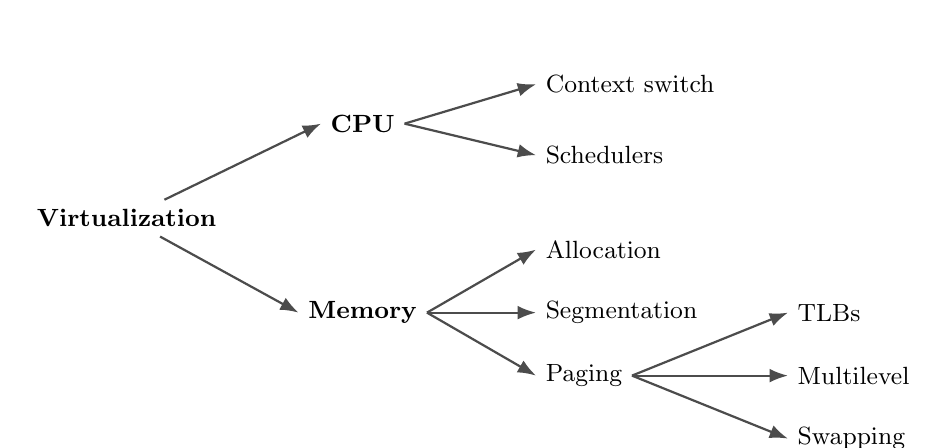
\begin{tikzpicture}[
  every node/.style={font=\small},
  arr/.style={-{Latex}, thick, black!70},
  level distance=1cm
]
  \node (v) at (0,0) {\textbf{Virtualization}};
  \node (cpu) at (3,1.2) {\textbf{CPU}};
  \node (mem) at (3,-1.2) {\textbf{Memory}};
  \node[anchor=west] (cs) at (5.2,1.7) {Context switch};
  \node[anchor=west] (sch) at (5.2,0.8) {Schedulers};
  \node[anchor=west] (al) at (5.2,-0.4) {Allocation};
  \node[anchor=west] (seg) at (5.2,-1.2) {Segmentation};
  \node[anchor=west] (pg) at (5.2,-2.0) {Paging};
  \node[anchor=west] (tlb) at (8.4,-1.2) {TLBs};
  \node[anchor=west] (ml) at (8.4,-2.0) {Multilevel};
  \node[anchor=west] (sw) at (8.4,-2.8) {Swapping};
  \draw[arr] (v) -- (cpu.west);
  \draw[arr] (v) -- (mem.west);
  \draw[arr] (cpu.east) -- (cs.west);
  \draw[arr] (cpu.east) -- (sch.west);
  \draw[arr] (mem.east) -- (al.west);
  \draw[arr] (mem.east) -- (seg.west);
  \draw[arr] (mem.east) -- (pg.west);
  \draw[arr] (pg.east) -- (tlb.west);
  \draw[arr] (pg.east) -- (ml.west);
  \draw[arr] (pg.east) -- (sw.west);
\end{tikzpicture}
\end{center}

\begin{itemize}
  \item \textbf{CPU virtualization:} context switches and schedulers give
        each process the illusion of its own CPU.
  \item \textbf{Memory virtualization:} allocation, segmentation, paging
        (with TLBs, multi-level page tables, and swapping) give each
        process the illusion of its own large private memory.
\end{itemize}

% ===========================================================================
\section{Motivation}
% ===========================================================================

\subsection{Overlapping CPU and I/O}

Recall from scheduling: process \(A\) alternates CPU bursts and disk I/O;
process \(B\) only computes.

\begin{center}
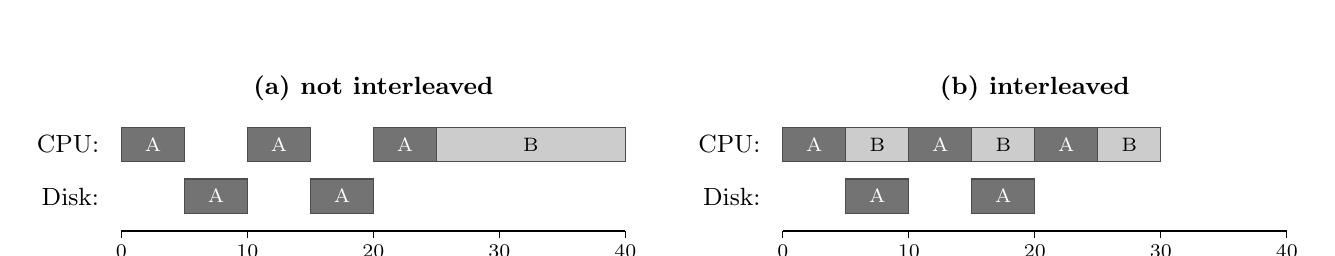
\begin{tikzpicture}[x=0.16cm, y=0.55cm,
  a/.style={fill=black!55, draw=black!70},
  b/.style={fill=black!20, draw=black!70},
  lab/.style={font=\scriptsize}]
  % (a) not interleaved
  \node[font=\small\bfseries] at (20,3.3) {(a) not interleaved};
  \node[anchor=east, font=\small] at (-1,2) {CPU:};
  \node[anchor=east, font=\small] at (-1,0.8) {Disk:};
  \foreach \s in {0,10,20} { \draw[a] (\s,1.6) rectangle (\s+5,2.4); \node[lab, white] at (\s+2.5,2) {A}; }
  \draw[b] (25,1.6) rectangle (40,2.4); \node[lab] at (32.5,2) {B};
  \foreach \s in {5,15} { \draw[a] (\s,0.4) rectangle (\s+5,1.2); \node[lab, white] at (\s+2.5,0.8) {A}; }
  \draw (0,0) -- (40,0);
  \foreach \t in {0,10,20,30,40} { \draw (\t,0) -- (\t,-0.15); \node[lab, below] at (\t,-0.1) {\t}; }

  % (b) interleaved
  \begin{scope}[xshift=8.4cm]
  \node[font=\small\bfseries] at (20,3.3) {(b) interleaved};
  \node[anchor=east, font=\small] at (-1,2) {CPU:};
  \node[anchor=east, font=\small] at (-1,0.8) {Disk:};
  \foreach \s in {0,10,20} { \draw[a] (\s,1.6) rectangle (\s+5,2.4); \node[lab, white] at (\s+2.5,2) {A}; }
  \foreach \s in {5,15,25} { \draw[b] (\s,1.6) rectangle (\s+5,2.4); \node[lab] at (\s+2.5,2) {B}; }
  \foreach \s in {5,15} { \draw[a] (\s,0.4) rectangle (\s+5,1.2); \node[lab, white] at (\s+2.5,0.8) {A}; }
  \draw (0,0) -- (40,0);
  \foreach \t in {0,10,20,30,40} { \draw (\t,0) -- (\t,-0.15); \node[lab, below] at (\t,-0.1) {\t}; }
  \end{scope}
\end{tikzpicture}
\end{center}

In (a) the CPU sits idle while \(A\) waits for the disk, and everything
finishes at time 40. In (b) the OS runs \(B\) while \(A\) does I/O; the
CPU never idles and the work finishes at time 30.

\begin{quizbox}[What if there is only one process?]
Interleaving needs \emph{another} runnable process to fill the gaps. If the
whole job is a \emph{single} process, there is nothing to switch to while
it waits for I/O --- and nothing else to put on a second CPU. We want a
way for \emph{one program} to have several independent streams of
execution. That is what this lecture builds.
\end{quizbox}

\subsection{CPU trends}

The slide shows the plot \textbf{Clock frequency vs.\ time} (MHz on a log
scale from 10 to 10\,000, years 1985--2010, chips from Intel, AMD, IBM,
DEC, Sun and others). Clock frequency rose exponentially until roughly
2005 and then \textbf{flattened} at a few GHz.

\begin{center}
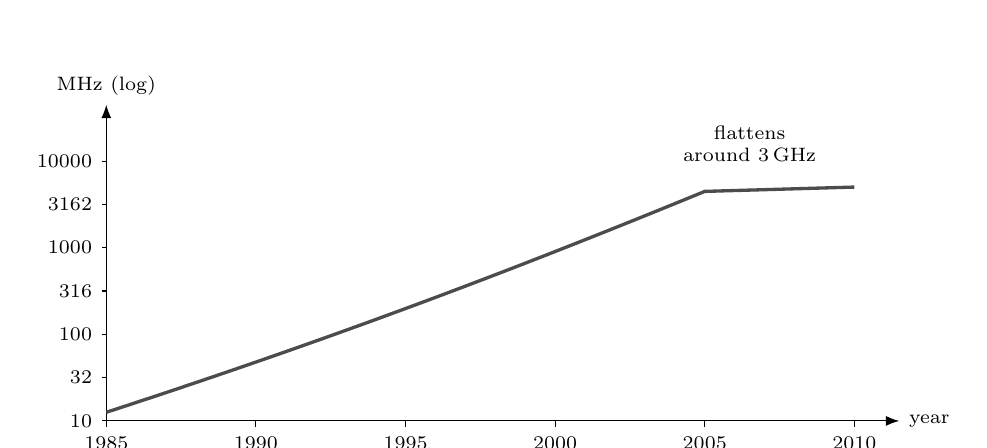
\begin{tikzpicture}[x=0.38cm, y=0.55cm]
  \draw[-{Latex}] (0,0) -- (26.5,0) node[right, font=\scriptsize] {year};
  \draw[-{Latex}] (0,0) -- (0,7.3) node[above, font=\scriptsize] {MHz (log)};
  \foreach \y/\l in {0/10,1/32,2/100,3/316,4/1000,5/3162,6/10000}
    { \draw (0,\y) -- (-0.15,\y) node[left, font=\scriptsize] {\l}; }
  \foreach \x/\l in {0/1985,5/1990,10/1995,15/2000,20/2005,25/2010}
    { \draw (\x,0) -- (\x,-0.15) node[below, font=\scriptsize] {\l}; }
  \draw[very thick, black!70] (0,0.2) .. controls (8,2.0) and (14,3.6) .. (20,5.3)
        -- (25,5.4);
  \node[font=\scriptsize, align=center] at (21.5,6.4) {flattens\\around 3\,GHz};
\end{tikzpicture}
\end{center}

\begin{keybox}[The future]
\begin{itemize}
  \item Same speed (clock frequency no longer increases).
  \item More cores.
\end{itemize}
So: \textbf{faster programs \(\Rightarrow\) concurrent execution}. A
program only gets faster on new hardware if it can run on many cores at
once.
\end{keybox}

% ===========================================================================
\section{Goal and two strategies}
% ===========================================================================

\begin{defbox}[Goal]
Write applications that fully utilize many CPUs.
\end{defbox}

\subsection{Strategy 1: many communicating processes}

Build applications from \textbf{many communicating processes}:
\begin{itemize}
  \item like Chrome (a process per tab);
  \item processes communicate via \texttt{pipe()} or similar.
\end{itemize}

\begin{center}
\renewcommand{\arraystretch}{1.2}
\begin{tabularx}{\textwidth}{@{}lX@{}}
  \toprule
  \textbf{Pro} & Don't need new abstractions --- processes already exist. \\
  \midrule
  \textbf{Cons} & \textbf{Cumbersome programming}: each process has its own
                  address space, so all sharing must be done by explicit
                  messages. \\
                & \textbf{Copying overheads}: data sent through a pipe is
                  copied from one address space, through the kernel, into
                  another. \\
                & \textbf{Expensive context switching}. \\
  \bottomrule
\end{tabularx}
\end{center}

\begin{keybox}[Why is a process context switch expensive?]
Switching between processes also switches \textbf{address spaces}: the
page-table base register (PTBR) changes, so TLB entries of the old process
are no longer usable (flushed, or kept apart by ASIDs) and the new
process starts with TLB misses and cold caches. This is the cost from the
TLB lecture.
\end{keybox}

\subsection{Strategy 2: threads}

\begin{defbox}[New abstraction: the thread]
Threads are just \textbf{like processes}, but they \textbf{share the
address space} (e.g.\ use the same page table).
\end{defbox}

A process can contain several threads. Each thread is an independent
stream of execution, but all of them see the same code, the same globals
and the same heap. Communication is just reading and writing memory --- no
copying --- and switching between threads of the same process does not
change the page table.

% ===========================================================================
\section{What state do threads share?}
% ===========================================================================

The slides answer this question piece by piece with two CPUs, each running
one thread of the same process.

\begin{center}
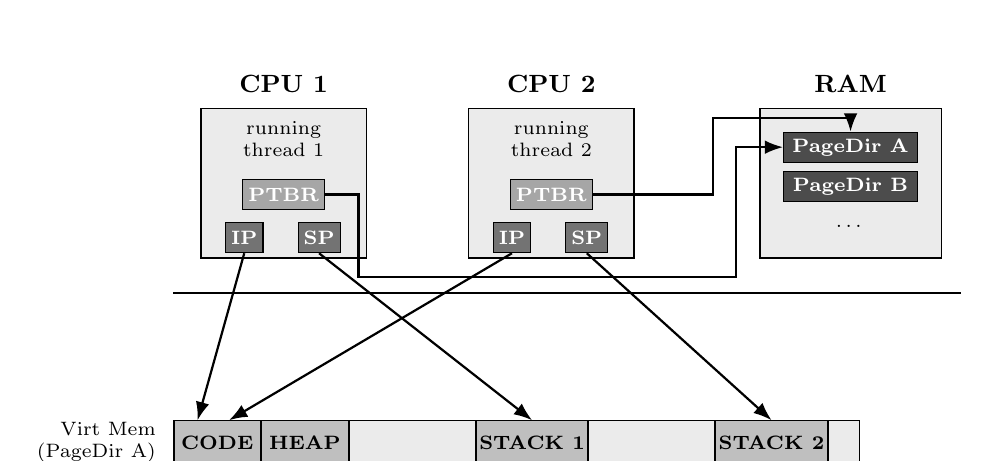
\begin{tikzpicture}[
  every node/.style={font=\small},
  cpu/.style={draw, fill=black!8, minimum width=2.1cm, minimum height=1.9cm, align=center, anchor=north},
  reg/.style={draw, fill=black!35, text=white, font=\scriptsize\bfseries, inner sep=2pt, minimum height=0.38cm},
  seg/.style={draw, minimum height=0.55cm, font=\scriptsize\bfseries, inner sep=1pt},
  arr/.style={-{Latex}, thick}
]
  \node[font=\small\bfseries] at (0,2.35) {CPU 1};
  \node[font=\small\bfseries] at (3.4,2.35) {CPU 2};
  \node[font=\small\bfseries] at (7.2,2.35) {RAM};
  \node[cpu] (c1) at (0,2.05) {};
  \node[cpu] (c2) at (3.4,2.05) {};
  \node[cpu, minimum width=2.3cm] (ram) at (7.2,2.05) {};
  \node[font=\scriptsize, align=center] at (0,1.65) {running\\thread 1};
  \node[font=\scriptsize, align=center] at (3.4,1.65) {running\\thread 2};
  \node[reg] (ptbr1) at (0,0.95) {PTBR};
  \node[reg] (ptbr2) at (3.4,0.95) {PTBR};
  \node[reg, fill=black!55] (ip1) at (-0.5,0.4) {IP};
  \node[reg, fill=black!55] (sp1) at (0.45,0.4) {SP};
  \node[reg, fill=black!55] (ip2) at (2.9,0.4) {IP};
  \node[reg, fill=black!55] (sp2) at (3.85,0.4) {SP};
  \node[reg, fill=black!70, minimum width=1.7cm] (pda) at (7.2,1.55) {PageDir A};
  \node[reg, fill=black!70, minimum width=1.7cm] (pdb) at (7.2,1.05) {PageDir B};
  \node[font=\scriptsize] at (7.2,0.55) {\ldots};
  \draw[thick] (-1.4,-0.3) -- (8.6,-0.3);

  \draw[arr] (ptbr1.east) -- (0.95,0.95) -- (0.95,-0.1) -- (5.75,-0.1)
        -- (5.75,1.55) -- (pda.west);
  \draw[arr] (ptbr2.east) -- (5.45,0.95) -- (5.45,1.92) -- (7.2,1.92) -- (pda.north);

  % virtual memory bar
  \node[font=\scriptsize, align=right, anchor=east] at (-1.5,-2.2) {Virt Mem\\(PageDir A)};
  \node[seg, fill=black!25, minimum width=1.1cm, anchor=west] (code) at (-1.4,-2.2) {CODE};
  \node[seg, fill=black!25, minimum width=1.1cm, right=0pt of code] (heap) {HEAP};
  \node[seg, fill=black!8, minimum width=1.6cm, right=0pt of heap] (g1) {};
  \node[seg, fill=black!25, minimum width=1.4cm, right=0pt of g1] (st1) {STACK 1};
  \node[seg, fill=black!8, minimum width=1.6cm, right=0pt of st1] (g2) {};
  \node[seg, fill=black!25, minimum width=1.4cm, right=0pt of g2] (st2) {STACK 2};
  \node[seg, fill=black!8, minimum width=0.4cm, right=0pt of st2] {};

  \draw[arr] (ip1.south) -- ($(code.north)+(-0.25,0)$);
  \draw[arr] (ip2.south) -- ($(code.north)+(0.15,0)$);
  \draw[arr] (sp1.south) -- (st1.north);
  \draw[arr] (sp2.south) -- (st2.north);
\end{tikzpicture}
\end{center}

\begin{enumerate}
  \item \textbf{Do threads share page directories?} \textbf{Yes.} Both
        CPUs' PTBRs point to the \emph{same} page directory. That is what
        ``share the address space'' means: one set of translations, so both
        threads see the same virtual memory (here called ``Virt Mem
        (PageDir A)'').
  \item \textbf{Do threads share the instruction pointer?} \textbf{No.}
        Both IPs point into the same CODE region, so threads \emph{share
        code}, but each thread may be executing \emph{different code at the
        same time} \(\Rightarrow\) \textbf{different instruction pointers}.
  \item \textbf{Do threads share the stack pointer?} \textbf{No.} Threads
        executing different functions need \textbf{different stacks}: each
        thread's SP points to its own stack (STACK 1, STACK 2) inside the
        one shared address space.
\end{enumerate}

\subsection{Thread vs.\ process}

\begin{center}
\renewcommand{\arraystretch}{1.2}
\begin{tabularx}{\textwidth}{@{}XX@{}}
  \toprule
  \textbf{Shared by all threads of a process} & \textbf{Private to each thread} \\
  \midrule
  \begin{itemize}[leftmargin=1.1em, topsep=0pt]
    \item Process ID (PID)
    \item Address space
      \begin{itemize}[topsep=0pt]
        \item code (instructions)
        \item most data (heap, globals)
      \end{itemize}
    \item Open file descriptors
    \item Current working directory
    \item User and group id
  \end{itemize}
  &
  \begin{itemize}[leftmargin=1.1em, topsep=0pt]
    \item Thread ID (TID)
    \item Set of registers, including the program counter and stack pointer
    \item Stack for local variables and return addresses
          (in the same address space)
  \end{itemize}
  \\
  \bottomrule
\end{tabularx}
\end{center}

\begin{warnbox}[Private stack, but not protected]
Each thread's stack is private in the sense that it uses it for its own
local variables, but it still lives in the \emph{shared} address space.
Nothing stops another thread from touching it through a pointer.
\end{warnbox}

% ===========================================================================
\section{Thread API (POSIX threads)}
% ===========================================================================

A variety of thread systems exist; we use \textbf{POSIX Pthreads}.
Common thread operations:
\begin{itemize}
  \item \textbf{Create} a thread,
  \item \textbf{Exit} from a thread,
  \item \textbf{Join} a thread (wait for it to finish) --- the thread
        analogue of \texttt{wait()} for processes.
\end{itemize}

\subsection{Thread creation}

\begin{lstlisting}[numbers=none]
#include <pthread.h>

int
pthread_create(      pthread_t*      thread,
               const pthread_attr_t* attr,
                     void*           (*start_routine)(void*),
                     void*           arg);
\end{lstlisting}

\begin{itemize}
  \item \texttt{thread}: used to interact with this thread (filled in by
        the call; pass it later to \texttt{pthread\_join}).
  \item \texttt{attr}: used to specify any attributes this thread might
        have, e.g.\ stack size, scheduling priority, \ldots\ (\texttt{NULL}
        = defaults).
  \item \texttt{start\_routine}: the function this thread starts running
        in. It takes one \texttt{void*} and returns a \texttt{void*}.
  \item \texttt{arg}: the argument to be passed to the function
        (\texttt{start\_routine}). A \textbf{void pointer} allows us to pass
        in \emph{any type} of argument.
\end{itemize}

\subsection{Wait for a thread to complete}

\begin{lstlisting}[numbers=none]
int pthread_join(pthread_t thread, void **value_ptr);
\end{lstlisting}

\begin{itemize}
  \item \texttt{thread}: specifies which thread \emph{to wait for}.
  \item \texttt{value\_ptr}: a pointer to the \textbf{return value}.
        Because the \texttt{pthread\_join()} routine changes the value, you
        need to \textbf{pass in a pointer} to that value --- hence
        \texttt{void **}.
\end{itemize}

\subsection{Example: two threads printing}

\begin{lstlisting}
#include <stdio.h>
//#include "mythreads.h"
#include <stdlib.h>
#include <pthread.h>

void *
mythread(void *arg) {
    printf("%s\n", (char *) arg);
    return NULL;
}

int
main(int argc, char *argv[])
{
    if (argc != 1) {
    fprintf(stderr, "usage: main\n");
    exit(1);
    }

    pthread_t p1, p2;
    printf("main: begin\n");
    pthread_create(&p1, NULL, mythread, "A");
    pthread_create(&p2, NULL, mythread, "B");
    // join waits for the threads to finish
    pthread_join(p1, NULL);
    pthread_join(p2, NULL);
    printf("main: end\n");
    return 0;
}
\end{lstlisting}

\begin{keybox}[What does it print?]
Always \texttt{main: begin} first and \texttt{main: end} last (the two
joins guarantee both threads are finished). In between, \texttt{A} and
\texttt{B} can appear in \textbf{either order}: once created, the threads
are scheduled independently, and creating \texttt{p1} first does not mean
it runs first.
\end{keybox}

\keepspace{26\baselineskip}
\subsection{Example: passing arguments to a thread}

More than one value is passed by packing them in a struct and passing a
pointer to it.

\begin{lstlisting}
#include <pthread.h>

typedef struct __myarg_t {
    int a;
    int b;
} myarg_t;

void *mythread(void *arg) {
    myarg_t *m = (myarg_t *) arg;
    printf("%d %d\n", m->a, m->b);
    return NULL;
}

int
main(int argc, char *argv[]) {
    pthread_t p;
    int rc;

    myarg_t args;
    args.a = 10;
    args.b = 20;
    rc = pthread_create(&p, NULL, mythread, &args);
    ...
}
\end{lstlisting}

The thread casts the \texttt{void *} back to \texttt{myarg\_t *} and
prints \texttt{10 20}.

\subsection{Example: returning a value from a thread}

\begin{lstlisting}[firstnumber=4]
#include <stdlib.h>

typedef struct __myarg_t {
    int a;
    int b;
} myarg_t;

typedef struct __myret_t {
    int x;
    int y;
} myret_t;

void *mythread(void *arg) {
    myarg_t *m = (myarg_t *) arg;
    printf("%d %d\n", m->a, m->b);
    myret_t *r = Malloc(sizeof(myret_t));
    r->x = 1;
    r->y = 2;
    return (void *) r;
}

int
main(int argc, char *argv[]) {
    pthread_t p;
    myret_t *m;

    myarg_t args = {10, 20};
    Pthread_create(&p, NULL, mythread, &args);
    Pthread_join(p, (void **) &m);
    printf("returned %d %d\n", m->x, m->y);
    free(m);
    return 0;
}
\end{lstlisting}

\begin{itemize}
  \item Output: \texttt{10 20}, then \texttt{returned 1 2}.
  \item The return value is \textbf{heap}-allocated (\texttt{Malloc}), so it
        is still valid after the thread finishes. The thread's own stack is
        gone once it exits, so it must never return a pointer to one of its
        local variables.
  \item \texttt{main} passes \texttt{(void **) \&m} so that
        \texttt{pthread\_join} can \emph{write} the returned pointer into
        \texttt{m}; \texttt{main} then frees it.
  \item The capitalised \texttt{Pthread\_create}, \texttt{Pthread\_join},
        \texttt{Malloc} are wrappers (from the \texttt{mythreads.h} header
        commented out in the first example) that call the real function and
        stop the program if it fails.
\end{itemize}

\keepspace{34\baselineskip}
\subsection{Example: exiting from a thread with \texttt{pthread\_exit}}

\begin{lstlisting}
#include <stdio.h>
#include <stdlib.h>
#include <pthread.h>
typedef struct __myret_t {
     int x;
    int y;
} myret;

void * mythread(void *arg) {
    printf("%s\n", (char *) arg);
    myret *r=malloc(sizeof(myret));
    r->x=10;r->y=5;
    pthread_exit((void *)r);
}

int
main(int argc, char *argv[])
{
    myret *m;
    if (argc != 1) {
    fprintf(stderr, "usage: main\n");
    exit(1);
    }

    pthread_t p1, p2;
    printf("main: begin\n");
    pthread_create(&p1, NULL, mythread, "A");
   // join waits for the threads to finish
    pthread_join(p1, (void **)&m);
    printf("main: return value from Thread\n  x=%d, y=%d\n",m->x,m->y );
    return 0;
}
\end{lstlisting}

\begin{itemize}
  \item \texttt{pthread\_exit(value)} ends the calling thread immediately;
        \texttt{value} becomes what \texttt{pthread\_join} receives. It is
        equivalent to \texttt{return value;} from the start routine, but it
        can also be called from deep inside other functions.
  \item Output: \texttt{main: begin}, \texttt{A}, then
        \texttt{main: return value from Thread} and \texttt{x=10, y=5}.
\end{itemize}

\keepspace{30\baselineskip}
% ===========================================================================
\section{Sharing data: the counter example}
% ===========================================================================

Two threads each add 1 to a \textbf{shared global} counter \texttt{max}
times. The final value \emph{should} be \(2 \times \texttt{max}\).

\begin{lstlisting}[firstnumber=4]
#include <pthread.h>

int max;
volatile int counter = 0; // shared global variable

void *
mythread(void *arg)
{
    char *letter = arg;
    int i; // stack (private per thread)
    printf("%s: begin [addr of i: %p]\n", letter, &i);
    for (i = 0; i < max; i++) {
    counter = counter + 1; // shared: only one
    }
    printf("%s: done\n", letter);
    return NULL;
}

int
main(int argc, char *argv[])
{
    if (argc != 2) {
    fprintf(stderr, "usage: main-first <loopcount>\n");
    exit(1);
    }
    max = atoi(argv[1]);

    pthread_t p1, p2;
    printf("main: begin [counter = %d] [%x]\n", counter,
        (unsigned int) &counter);
    Pthread_create(&p1, NULL, mythread, "A");
    Pthread_create(&p2, NULL, mythread, "B");
    // join waits for the threads to finish
    Pthread_join(p1, NULL);
    Pthread_join(p2, NULL);
    printf("main: done\n [counter: %d]\n [should: %d]\n",
        counter, max*2);
    return 0;
}
\end{lstlisting}

\begin{itemize}
  \item \texttt{counter} and \texttt{max} are globals: \textbf{one} copy,
        shared by both threads.
  \item \texttt{i} is a local variable: it lives on each thread's
        \textbf{own stack}, so each thread has its own \texttt{i}.
  \item \texttt{volatile} tells the compiler to really load and store
        \texttt{counter} in memory on every iteration (not keep it in a
        register). It does \emph{not} make the update atomic.
\end{itemize}

\keepspace{28\baselineskip}
\subsection{Running it three times with \texttt{max} = 100000}

\begin{lstlisting}[style=term]
/Users/Minati/Documents/my-computer/reads-Intro# ./t1 100000
main: begin [counter = 0] [d7e7048]
A: begin [addr of i: 0x700009567edc]
B: begin [addr of i: 0x7000095eaedc]
A: done
B: done
main: done
 [counter: 114719]
 [should: 200000]
/Users/Minati/Documents/my-computer/reads-Intro# ./t1 100000
main: begin [counter = 0] [17fc048]
A: begin [addr of i: 0x700001366edc]
B: begin [addr of i: 0x7000013e9edc]
B: done
A: done
main: done
 [counter: 107303]
 [should: 200000]
/Users/Minati/Documents/my-computer/reads-Intro# ./t1 100000
main: begin [counter = 0] [9c98048]
A: begin [addr of i: 0x70000833eedc]
B: begin [addr of i: 0x7000083c1edc]
A: done
B: done
main: done
 [counter: 113941]
 [should: 200000]
\end{lstlisting}

\begin{warnbox}[Observations]
\begin{itemize}
  \item The answer is \textbf{wrong} (should be 200000) and
        \textbf{different on every run}: 114719, 107303, 113941.
  \item The two \texttt{addr of i} values differ in each run: the two
        threads really do have separate stacks.
  \item Even the order of \texttt{A: done} / \texttt{B: done} changes between
        runs.
\end{itemize}
Why? Because \texttt{counter = counter + 1} is \textbf{not one
instruction}.
\end{warnbox}

% ===========================================================================
\section{Why the counter is wrong: thread schedules}
% ===========================================================================

\texttt{counter = counter + 1}, with \texttt{counter} at address
\texttt{0x9cd4}, compiles to three x86 instructions:

\begin{center}
\renewcommand{\arraystretch}{1.12}
\begin{tabular}{@{}lll@{}}
  \toprule
  \textbf{Address} & \textbf{Instruction} & \textbf{Effect} \\
  \midrule
  \texttt{0x195} & \texttt{mov 0x9cd4, \%eax} & load \texttt{counter} from memory into \eax \\
  \texttt{0x19a} & \texttt{add \$0x1, \%eax}  & \(\eax \gets \eax + 1\) \\
  \texttt{0x19d} & \texttt{mov \%eax, 0x9cd4} & store \eax\ back to \texttt{counter} \\
  \bottomrule
\end{tabular}
\end{center}

Each thread has its own registers. When the OS switches threads, it saves
the running thread's \eax\ and \rip\ in that thread's \textbf{control
block} (shown on the slides as ``process control blocks'' for Thread 1 and
Thread 2) and restores the other thread's. Memory (\texttt{0x9cd4}) is
shared. Initially \(\texttt{counter} = 100\).

\subsection{Thread schedule \#1: no interleaving inside the update}

\begin{center}
\renewcommand{\arraystretch}{1.1}
\setlength{\tabcolsep}{5pt}
\begin{tabular}{@{}clccc|cc@{}}
  \toprule
  & & \multicolumn{3}{c|}{\textbf{CPU state after}} & \multicolumn{2}{c}{\textbf{Saved in control block}} \\
  \textbf{Runs} & \textbf{Instruction} & \texttt{0x9cd4} & \eax & \rip & \textbf{T1} (\eax, \rip) & \textbf{T2} (\eax, \rip) \\
  \midrule
  --  & (initial)                   & 100 & ?   & 0x195 & ?, 0x195   & ?, 0x195 \\
  T1  & \texttt{mov 0x9cd4, \%eax}  & 100 & 100 & 0x19a & & \\
  T1  & \texttt{add \$0x1, \%eax}   & 100 & 101 & 0x19d & & \\
  T1  & \texttt{mov \%eax, 0x9cd4}  & 101 & 101 & 0x1a2 & & \\
  \midrule
  \multicolumn{7}{c}{\textit{thread context switch: save T1, restore T2}} \\
  \midrule
  T2  & (restored)                  & 101 & ?   & 0x195 & 101, 0x1a2 & ?, 0x195 \\
  T2  & \texttt{mov 0x9cd4, \%eax}  & 101 & 101 & 0x19a & & \\
  T2  & \texttt{add \$0x1, \%eax}   & 101 & 102 & 0x19d & & \\
  T2  & \texttt{mov \%eax, 0x9cd4}  & 102 & 102 & 0x1a2 & & \\
  \bottomrule
\end{tabular}
\end{center}

Final value \textbf{102}: correct. T1 finished all three instructions
before T2 read the counter.

\subsection{Thread schedule \#2: switch in the middle}

\begin{center}
\renewcommand{\arraystretch}{1.1}
\setlength{\tabcolsep}{5pt}
\begin{tabular}{@{}clccc|cc@{}}
  \toprule
  & & \multicolumn{3}{c|}{\textbf{CPU state after}} & \multicolumn{2}{c}{\textbf{Saved in control block}} \\
  \textbf{Runs} & \textbf{Instruction} & \texttt{0x9cd4} & \eax & \rip & \textbf{T1} (\eax, \rip) & \textbf{T2} (\eax, \rip) \\
  \midrule
  --  & (initial)                   & 100 & ?   & 0x195 & ?, 0x195   & ?, 0x195 \\
  T1  & \texttt{mov 0x9cd4, \%eax}  & 100 & 100 & 0x19a & & \\
  T1  & \texttt{add \$0x1, \%eax}   & 100 & 101 & 0x19d & & \\
  \midrule
  \multicolumn{7}{c}{\textit{thread context switch: save T1 (101, 0x19d), restore T2}} \\
  \midrule
  T2  & (restored)                  & 100 & ?   & 0x195 & 101, 0x19d & ?, 0x195 \\
  T2  & \texttt{mov 0x9cd4, \%eax}  & 100 & 100 & 0x19a & & \\
  T2  & \texttt{add \$0x1, \%eax}   & 100 & 101 & 0x19d & & \\
  T2  & \texttt{mov \%eax, 0x9cd4}  & 101 & 101 & 0x1a2 & & \\
  \midrule
  \multicolumn{7}{c}{\textit{thread context switch: save T2 (101, 0x1a2), restore T1}} \\
  \midrule
  T1  & (restored)                  & 101 & 101 & 0x19d & 101, 0x19d & 101, 0x1a2 \\
  T1  & \texttt{mov \%eax, 0x9cd4}  & \textbf{101} & 101 & 0x1a2 & & \\
  \bottomrule
\end{tabular}
\end{center}

\begin{warnbox}[WRONG result! Final value of balance is 101]
Both threads read the \emph{old} value 100 before either wrote back. Each
computed 101 in its own private \eax, and each stored 101. One increment
is \textbf{lost}. This is exactly what happened tens of thousands of times
in the 200000-iteration run.
\end{warnbox}

% ===========================================================================
\newpage
\section{Timeline view}
% ===========================================================================

Now Thread 1 adds 1 and Thread 2 adds 2 to a shared variable at address
\texttt{0x123}. Each thread runs three instructions:
\begin{center}
\begin{tabular}{@{}ll@{}}
  \textbf{Thread 1} & \textbf{Thread 2} \\
  \texttt{mov 0x123, \%eax} & \texttt{mov 0x123, \%eax} \\
  \texttt{add \%0x1, \%eax} & \texttt{add \%0x2, \%eax} \\
  \texttt{mov \%eax, 0x123} & \texttt{mov \%eax, 0x123} \\
\end{tabular}
\end{center}
(The slides write the constants as \texttt{\%0x1} and \texttt{\%0x2}; they
mean the immediates \texttt{\$0x1} and \texttt{\$0x2}, as in
\texttt{add \$0x1, \%eax} above.) The correct total added is \(1+2=3\). Time flows downward in each table;
a row belongs to whichever thread is running.

\begin{solbox}[How much is added to the shared variable? The five interleavings on the slides]
\renewcommand{\arraystretch}{1.05}
\small
\begin{tabular}{@{}p{0.47\textwidth}p{0.47\textwidth}@{}}
\textbf{(a)} &
\textbf{(b)} \\
\begin{tabular}{@{}ll@{}}
  \toprule \textbf{Thread 1} & \textbf{Thread 2} \\ \midrule
  \texttt{mov 0x123, \%eax} & \\
  \texttt{add \%0x1, \%eax} & \\
  \texttt{mov \%eax, 0x123} & \\
  & \texttt{mov 0x123, \%eax} \\
  & \texttt{add \%0x2, \%eax} \\
  & \texttt{mov \%eax, 0x123} \\ \bottomrule
\end{tabular}
&
\begin{tabular}{@{}ll@{}}
  \toprule \textbf{Thread 1} & \textbf{Thread 2} \\ \midrule
  \texttt{mov 0x123, \%eax} & \\
  \texttt{add \%0x1, \%eax} & \\
  & \texttt{mov 0x123, \%eax} \\
  \texttt{mov \%eax, 0x123} & \\
  & \texttt{add \%0x2, \%eax} \\
  & \texttt{mov \%eax, 0x123} \\ \bottomrule
\end{tabular}
\\[0.3em]
Added: \textbf{3 --- correct.} T1 finishes before T2 reads. &
Added: \textbf{2 --- incorrect!} T2 read the old value before T1
stored, so T2's store of \(v+2\) overwrites T1's \(v+1\). \\[1.0em]

\textbf{(c)} &
\textbf{(d)} \\
\begin{tabular}{@{}ll@{}}
  \toprule \textbf{Thread 1} & \textbf{Thread 2} \\ \midrule
  & \texttt{mov 0x123, \%eax} \\
  \texttt{mov 0x123, \%eax} & \\
  & \texttt{add \%0x2, \%eax} \\
  \texttt{add \%0x1, \%eax} & \\
  & \texttt{mov \%eax, 0x123} \\
  \texttt{mov \%eax, 0x123} & \\ \bottomrule
\end{tabular}
&
\begin{tabular}{@{}ll@{}}
  \toprule \textbf{Thread 1} & \textbf{Thread 2} \\ \midrule
  & \texttt{mov 0x123, \%eax} \\
  & \texttt{add \%0x2, \%eax} \\
  & \texttt{mov \%eax, 0x123} \\
  \texttt{mov 0x123, \%eax} & \\
  \texttt{add \%0x1, \%eax} & \\
  \texttt{mov \%eax, 0x123} & \\ \bottomrule
\end{tabular}
\\[0.3em]
Added: \textbf{1 --- incorrect!} Both read \(v\); T2 stores \(v+2\), then
T1 overwrites it with \(v+1\). &
Added: \textbf{3 --- correct.} T2 finishes completely before T1 starts.
\\[1.0em]

\textbf{(e)} & \\
\begin{tabular}{@{}ll@{}}
  \toprule \textbf{Thread 1} & \textbf{Thread 2} \\ \midrule
  & \texttt{mov 0x123, \%eax} \\
  & \texttt{add \%0x2, \%eax} \\
  \texttt{mov 0x123, \%eax} & \\
  \texttt{add \%0x1, \%eax} & \\
  \texttt{mov \%eax, 0x123} & \\
  & \texttt{mov \%eax, 0x123} \\ \bottomrule
\end{tabular}
&
\\[0.3em]
Added: \textbf{2 --- incorrect!} Both read \(v\); T1 stores \(v+1\), then
T2 overwrites it with \(v+2\). & \\
\end{tabular}
\end{solbox}

\begin{keybox}[Pattern]
The result is correct only when one thread's three instructions run
\emph{entirely before} the other thread's load. If both threads load the
old value, the \textbf{last store wins} and the other update is lost: the
total added is either 1 or 2 depending on who stores last.
\end{keybox}

% ===========================================================================
\section{Non-determinism}
% ===========================================================================

\begin{defbox}[Concurrency leads to non-deterministic results]
\begin{itemize}
  \item \textbf{Not deterministic result:} different results even with the
        same inputs.
  \item This is a \textbf{race condition}: the result depends on the timing
        (the ``race'') between threads.
\end{itemize}
\end{defbox}

\begin{itemize}
  \item Whether the bug manifests \textbf{depends on the CPU schedule!}
  \item \textbf{Passing tests means little}: the bad interleaving might
        just not have happened during the test run.
  \item \textbf{How to program:} imagine the scheduler is
        \textbf{malicious}. Assume the scheduler will pick a bad ordering at
        some point\ldots
\end{itemize}

% ===========================================================================
\section{What do we want?}
% ===========================================================================

We want the 3 instructions to execute as an \textbf{uninterruptable
group}. That is, we want them to be \textbf{atomic}.

\begin{center}
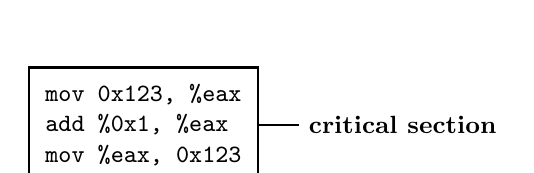
\begin{tikzpicture}
  \node[draw, thick, inner sep=6pt, align=left, font=\ttfamily\small] (cs) {
    mov 0x123, \%eax\\
    add \%0x1, \%eax\\
    mov \%eax, 0x123};
  \draw[thick] (cs.east) -- ++(0.5,0) node[right, font=\small] {\textbf{critical section}};
\end{tikzpicture}
\end{center}

\begin{defbox}[Critical section and mutual exclusion]
A \textbf{critical section} is a piece of code that accesses a shared
variable and must not be executed concurrently by more than one thread.

More generally: we need \textbf{mutual exclusion} for critical sections.
If process \(A\) is in critical section \(C\), process \(B\) can't be
(it is okay if other processes do unrelated work).
\end{defbox}

With atomicity, only interleavings (a) and (d) of the timeline are
possible, and the result is always correct.

% ===========================================================================
\section{Summary}
% ===========================================================================

\begin{keybox}[Conclusions]
\begin{itemize}
  \item \textbf{Concurrency} is needed to obtain high performance by
        utilizing multiple cores.
  \item \textbf{Threads} are multiple execution streams within a single
        process or address space (they share the PID and address space;
        each has its own registers and stack).
  \item \textbf{Context switches within a critical section} can lead to
        non-deterministic bugs (\textbf{race conditions}).
  \item Use \textbf{locks} to provide \textbf{mutual exclusion}.
\end{itemize}
\end{keybox}

\begin{center}
\renewcommand{\arraystretch}{1.18}
\begin{tabular}{@{}lll@{}}
  \toprule
  & \textbf{Processes (strategy 1)} & \textbf{Threads (strategy 2)} \\
  \midrule
  Address space        & separate             & shared (same page table) \\
  Communication        & \texttt{pipe()}, copying & shared memory \\
  Context switch       & expensive (new PTBR) & cheaper (same PTBR) \\
  Registers / stack    & own                  & own \\
  New abstraction?     & no                   & yes \\
  Danger               & ---                  & race conditions on shared data \\
  \bottomrule
\end{tabular}
\end{center}

\begin{warnbox}[Next]
How to actually build \textbf{locks} that make critical sections atomic.
\end{warnbox}

\end{document}
